\documentclass[a4paper,10pt]{report}
\usepackage{ucs}
\usepackage[utf8]{inputenc}
\usepackage[francais]{babel}
\usepackage{fontenc}
\usepackage{graphicx}
\usepackage{pdfpages}
\usepackage{float}
\usepackage{dirtree}
\usepackage{titlesec}
\usepackage[hidelinks]{hyperref}
\usepackage{caption}
\usepackage{textcomp}
\author{}

\date{31/05/2018}

\title{Documentation Ancor2}
\setcounter{secnumdepth}{1}
\setcounter{tocdepth}{4}
\titleformat{\chapter}
  {\Large\bfseries} % format
  {}                % label
  {0pt}             % sep
  {\huge}   
\newcommand{\sectionbreak}{\clearpage}
\titlespacing\chapter{0pt}{0pt plus 0pt minus 2pt}{0pt plus 2pt minus 2pt}


\begin{document}
 \maketitle
 \tableofcontents
 \chapter{Informations générales}
 \subsection{Dépôts git}
 \begin{description}
  \item [Alexis] https://bitbucket.org/Slayug/ancortodemocrat.git
  \item [Augustin] https://gitlab.com/augustinvoima/ancor2.git
 \end{description}
 
 \subsection{Données des expériences}
 https://drive.google.com/drive/u/0/folders/14mp2w690RVP6yh3H2dmxkYIeB-LMa2E2
 \subsection{Documentation}
 https://docs.google.com/document/d/1vJP4o1z3eCfZSxo88vZTlS0OpT54B1Zu-Nfq4naSlWc/edit?usp=sharing
 
 \subsection{Dépendances}
 \begin{description}
  \item [git submodule] \begin{itemize}
                         \item reference-coreference-scorers
                        \end{itemize}

  \item [maven] \begin{description}
                 \item [javax.xml.bind] Parser XML
                 \item [log4j] Sortie text
                 \item [nz.ac.waikato.cms.weka] Classification
                 \item [org.annolab.tt4j] TreeTager: gestion des annotations \emph{part-of-speech}
                 \item [commons-cli] Gestion des arguments en ligne de commande (Remplacement de l'ancienne gestion des arguments à faire)
                 \item [commons-io] Gestion des Fichiers
                 \item [org.odftoolkit] Gestion des fichiers OpenDocument (sortie des résultats pour les expériences, en cours de dvlp)
                 
                \end{description}
                

 \end{description}


 \pagebreak
 \chapter{Processus}
  \section{Appel des fonctionnalités}
  
    \noindent
    \includegraphics[width=\textwidth,keepaspectratio]{ancortodemocrat.pdf}  
  
 \pagebreak
 \chapter{Architecture du projet}
  \begin{figure}[!htbp]
    \caption*{Packages du projet}
    \dirtree{%
      .1 com.democrat.
	.2 com.democrat.ancortodemocrat.
	  .3 com.democrat.ancortodemocrat.element.
	  .3 com.democrat.ancortodemocrat.feature.
	  .3 com.democrat.ancortodemocrat.positioning.
	  .3 com.democrat.ancortodemocrat.treetager.	
	.2 com.democrat.classification.
	.2 com.democrat.expes.
	  .3 com.democrat.expes.rjc18.
	  }
  \end{figure}
 \pagebreak
  \begin{section}{com.democrat.ancortodemocrat}  
    \begin{figure}[!htbp]
      \caption*{sous-packages}
      \dirtree{%
	  .1 com.democrat.ancortodemocrat.
	    .2 com.democrat.ancortodemocrat.element.
	    .2 com.democrat.ancortodemocrat.feature.
	    .2 com.democrat.ancortodemocrat.positioning.
	    .2 com.democrat.ancortodemocrat.treetager.	
	    }
    \end{figure}
     \begin{figure}[!htbp]      
      \advance\leftskip-2cm
      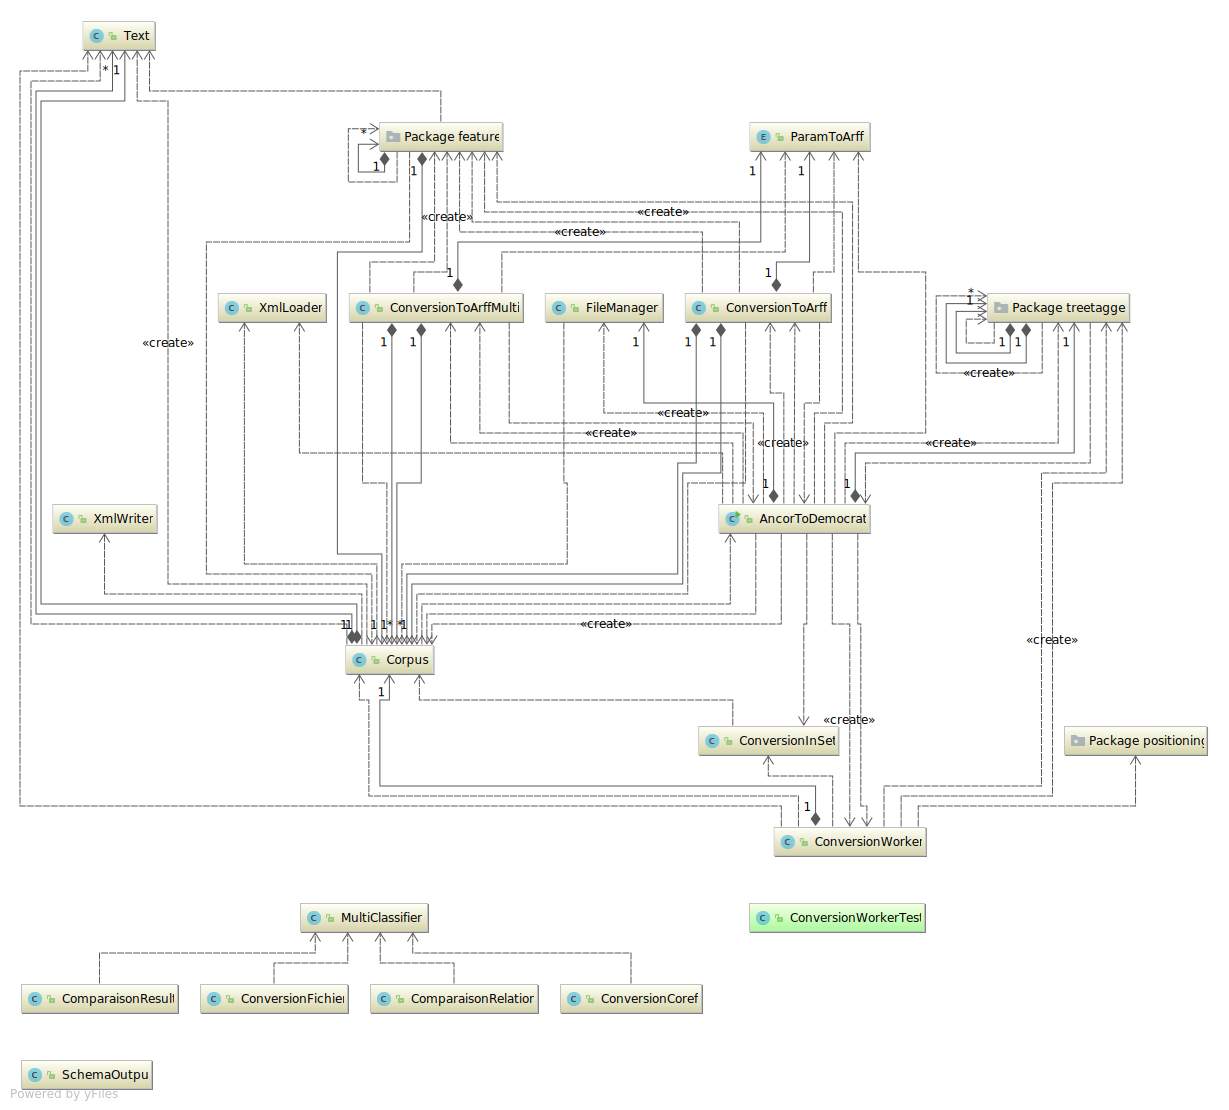
\includegraphics[width=1.45\linewidth,keepaspectratio]{Package_ancortodemocrat.pdf}
     \end{figure}
     \vfill
  \pagebreak
  \subsection{com.democrat.ancortodemocrat.element}
     \begin{figure}[!htbp]      
      \advance\leftskip-4cm
      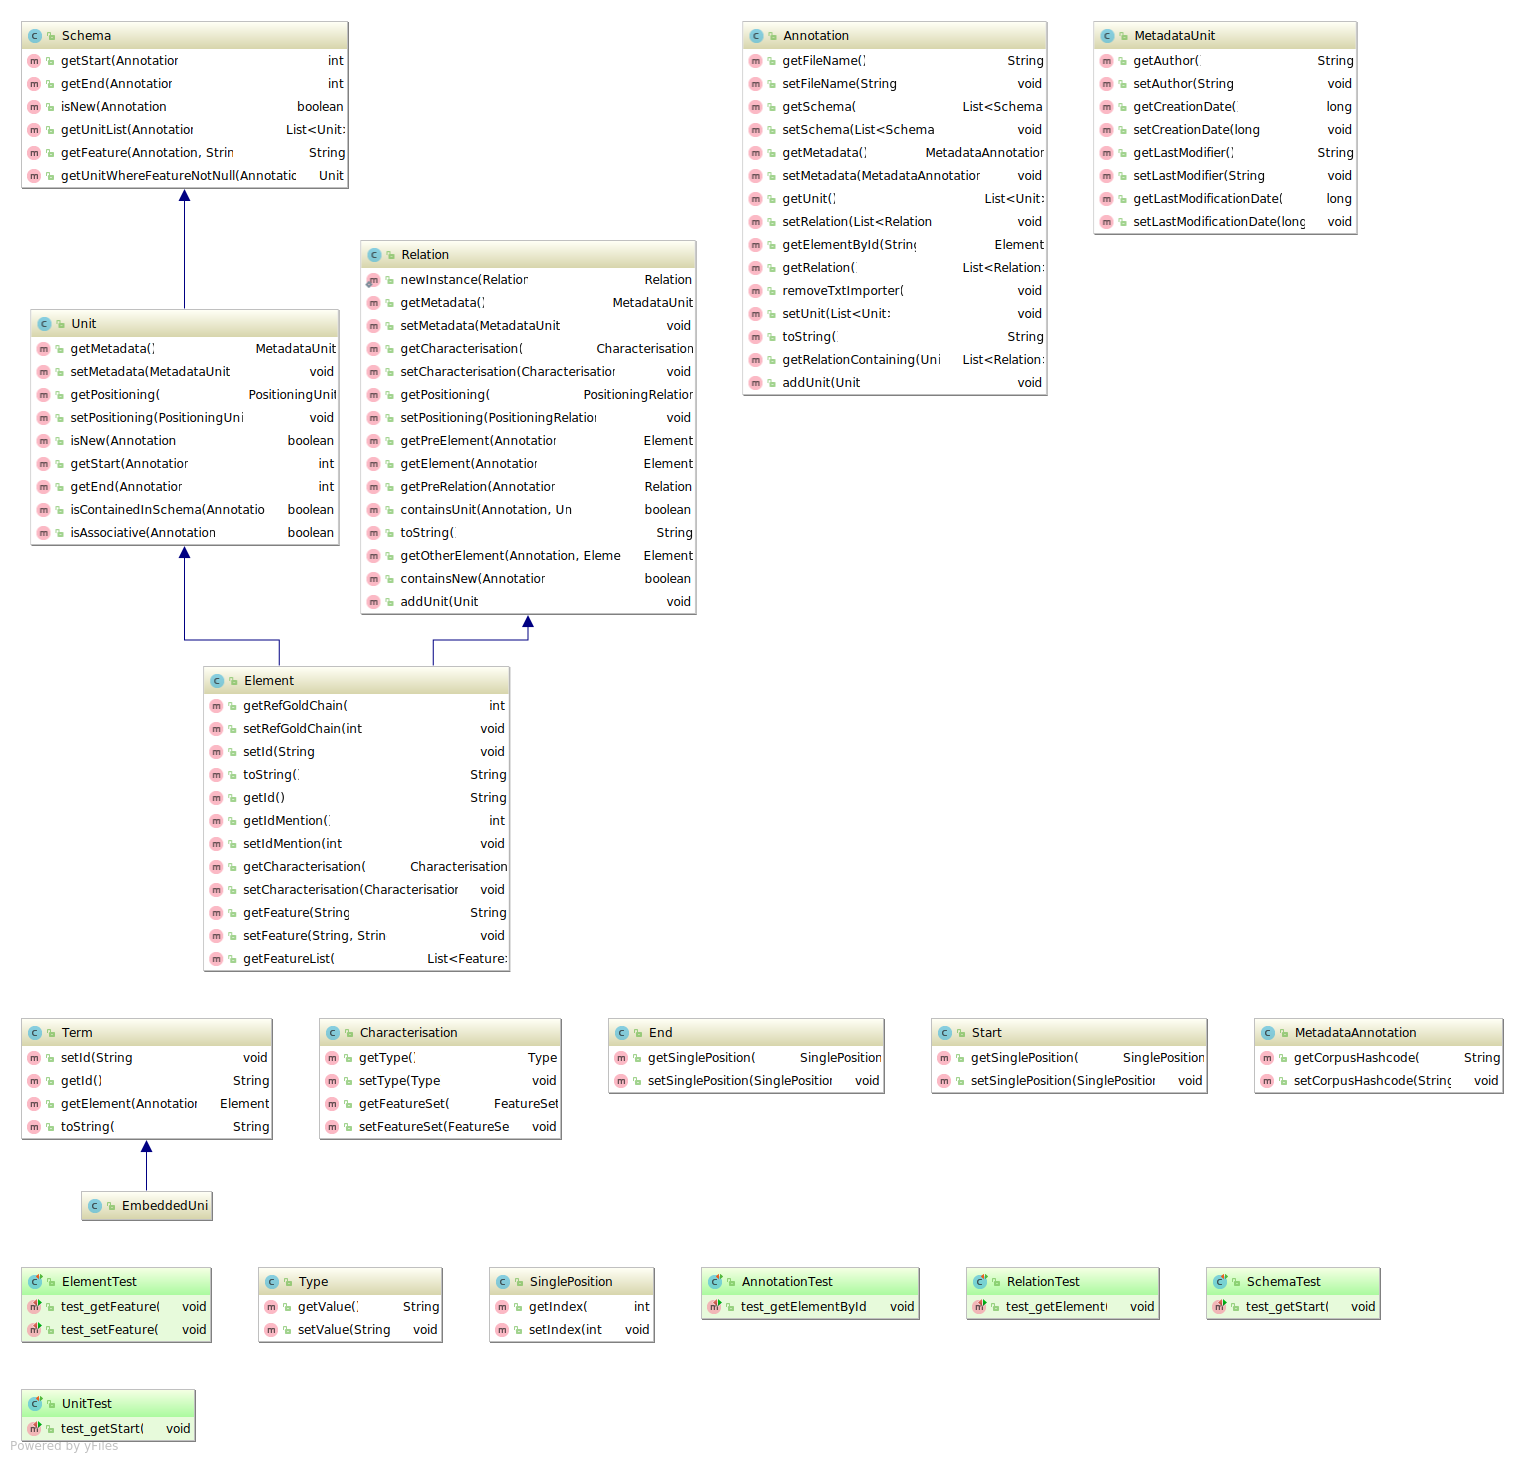
\includegraphics[width=1.6\linewidth, keepaspectratio]{Package_element.pdf}
     \end{figure}
  
  \pagebreak
  \begin{subsection}{com.democrat.ancortodemocrat.feature}  
     \begin{figure}[!htbp]      
\centering	
      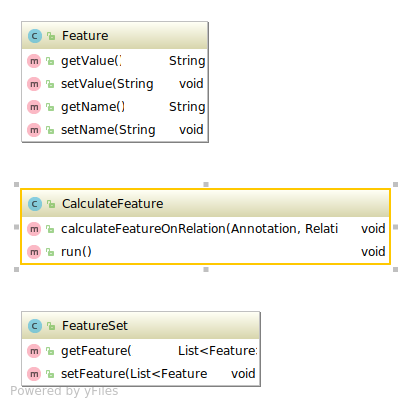
\includegraphics[width=0.7\linewidth, keepaspectratio]{Package_feature.pdf}
     \end{figure}
     \vfill
  \end{subsection}
  
  \pagebreak
  \begin{subsection}{com.democrat.ancortodemocrat.positioning}  
     \begin{figure}[!htbp]      
\centering
      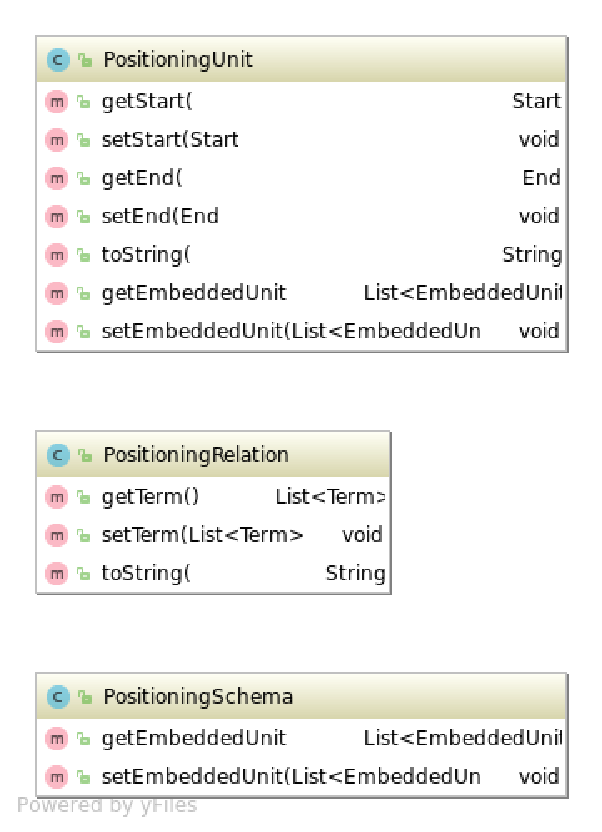
\includegraphics[width=0.7\linewidth, keepaspectratio]{Package_positioning.pdf}
     \end{figure}
     
  \end{subsection}  
  \pagebreak
  \begin{subsection}{com.democrat.ancortodemocrat.treetagger}  
     \begin{figure}[!htbp]      
      \centering
      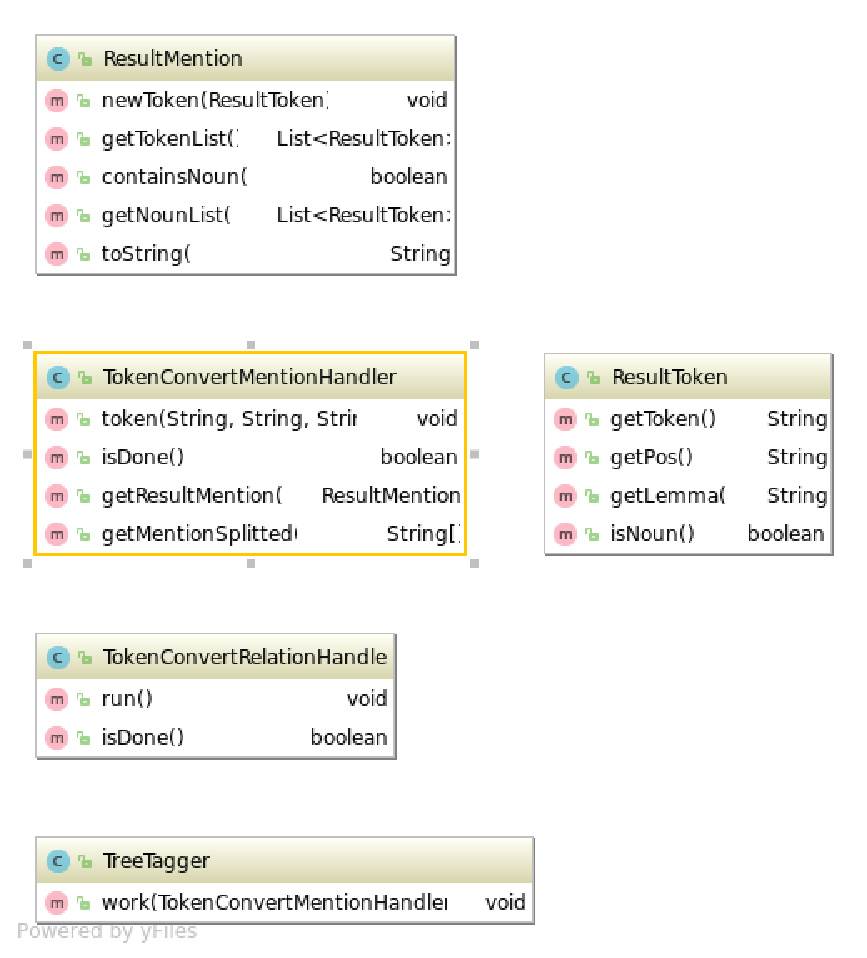
\includegraphics[width=0.7\linewidth, keepaspectratio]{Package_treetagger.pdf}
     \end{figure}
     \vfill
  \end{subsection}
 \end{section}
 
 \pagebreak
 \begin{section}{com.democrat.classification}  
     \begin{figure}[!htbp]      
      \centering
      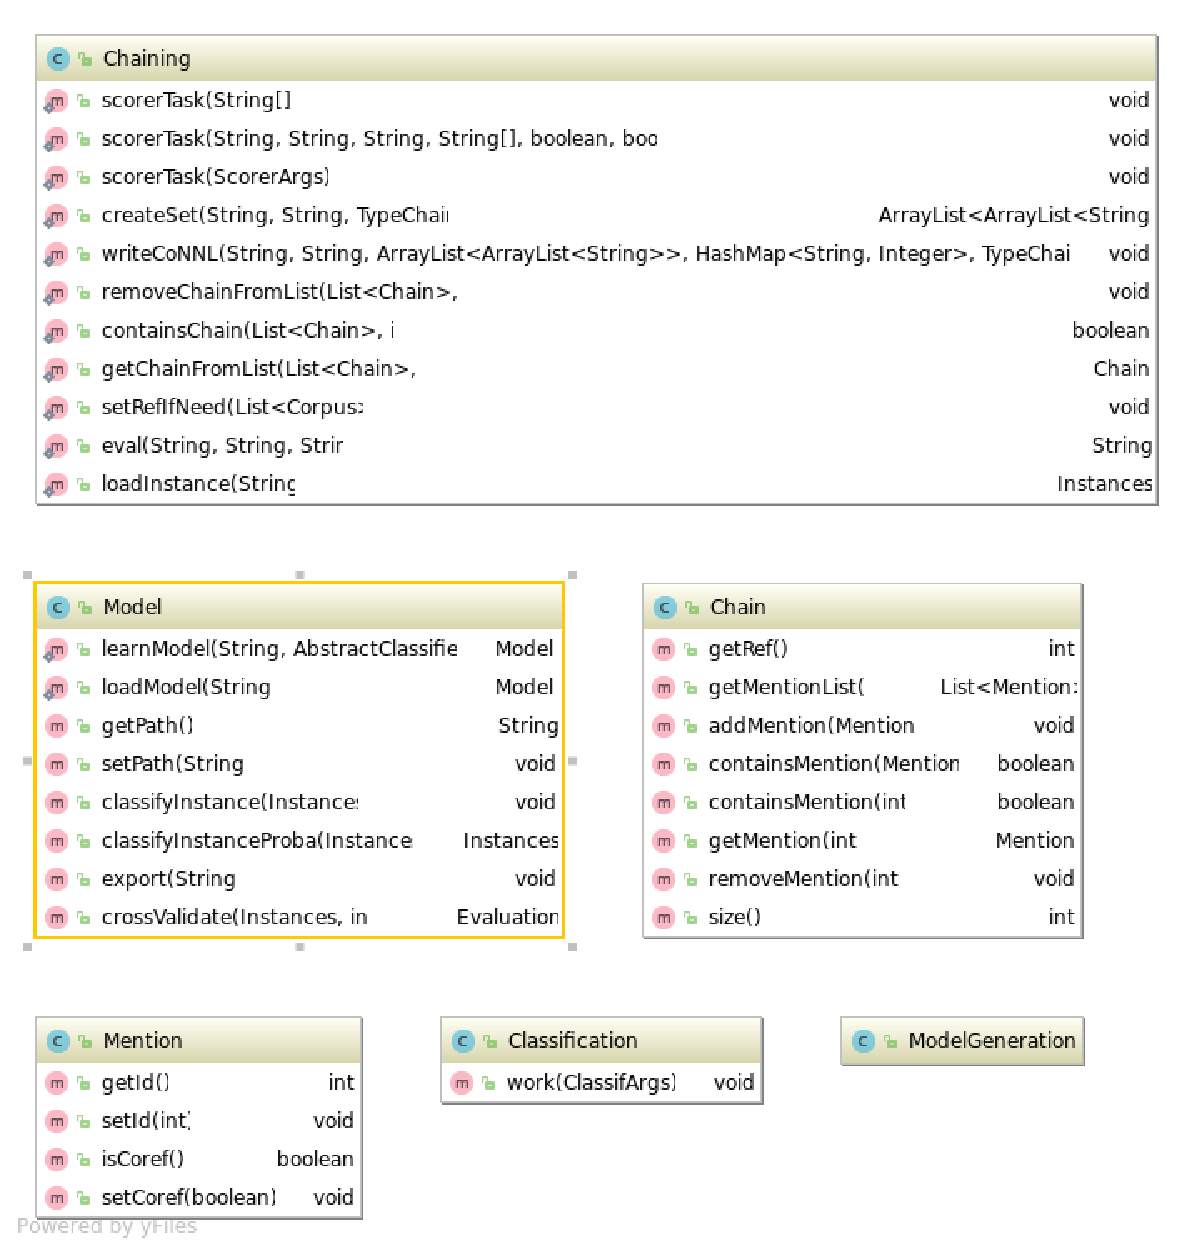
\includegraphics[width=1.2\linewidth, keepaspectratio]{Package_classification.pdf}
     \end{figure}
     \vfill
  \end{section}
  
 \pagebreak
 \begin{section}{com.democrat.expes}  
     \begin{figure}[!htbp]      
      \centering
      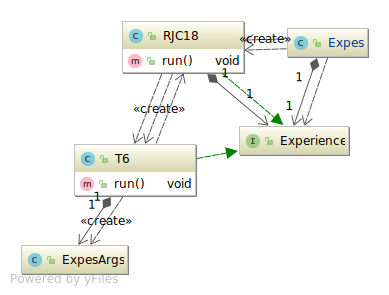
\includegraphics[width=0.7\linewidth, keepaspectratio]{Package_expes.pdf}
     \end{figure}
     \vfill
  \end{section}
  \chapter{Entrées - Sorties}
  \section{Calcul des features}

    \begin{description}
     \item [Entrée:] Corpus source: chemin/vers/Ancor
		    \begin{figure}[h!b]		      
		      \dirtree{%
			.1 chemin/vers/corpus/Ancor.
			  .2 aa\_fichiers.
			    .3 *.aa.
			  .2 ac\_fichiers.
			    .3 *.ac.
		      }
		    \end{figure}
      \item[Sortie:] Corpus avec nouveaux features calculés: chemin/vers/features	
		    \begin{figure}[h!b]		      
		      \dirtree{%
			.1 chemin/vers/features.
			  .2 aa\_fichiers.
			    .3 *.aa.
			  .2 ac\_fichiers.
			    .3 *.ac.
		      }
		    \end{figure}
    \end{description}
    \paragraph{Etapes du calcul des features}
    \begin{verbatim}
	com.democrat.AncorToDemocrat::generateFeature(corpus, output){
	    Pour chaque annotation du corpus:
	        ConversionInSet.toSetFrom{Chain/FirstMention}(annotation) // Genère le feature REF
	    CalculateFeature::new(corpus,output){
	        Pour chaque annotation du corpus:
	        calculateNewFeature(annotation)
	        calculateFeatureOnRelation(annotation)
	        corpus.export(output)
	    }
	}
    \end{verbatim}

    

  \section{Génération des arff}
    \begin{description}
     \item [Entrée:] Corpus contenant tous les features: chemin/vers/features			    
     \item [Sortie:] nomfichier
	  \itemize
	    \item nomfichier(date).arff \textrightarrow  Contient toutes les instances
	    \item nomfichier(date).idff \textrightarrow  Contient les identifiants de chaque instance et des mentions qui les composent
    \end{description}
    \paragraph{Etapes génération Arff}
    \begin{verbatim}
     com.democrat.ancortodemocrat.ConversionToArff::work(){
        sortInstance(){
            Pour chaque corpus:
              Pour chaque annotation du corpus:
                 Pour chaque relation de l'annotation:
                    positiveRelationSelected.put(relation)
                    generateNegativeRelation(corpus,annotation, relation){
                       Pour chaque relation négative à générer:
                          newrelation = deux mentions au hasard qui ont
                                        un champ REF différent
                          negativeRelationSelected.put(newrelation)                                 
                   }
        }
        selectInstance(){
            restriction nb_pos et nb_neg en fonction 
               du nombre d'instances dans le corpus 
               et en conservant le ratio
            mélange aléatoire de la liste des instances positives // à modifier
            mélange aléatoire de la liste des instances négatives            
        }
        writeInstance()       
     }
    \end{verbatim}

  
  \section{Génération du model}
    \begin{description}
     \item[Entrée:] Corpus d'apprentissage et de test
     \begin{itemize}
	  \item train.arff 
	  \item test.arff
     \end{itemize}
     \item[Sortie:] Model
    \end{description}
    \paragraph{Etapes génération du model}
    \begin{verbatim}
     com.democrat.classification.ModelGeneration::execute( classifierclass, args ){
         AbstractClassifier.runClassifier(classifierclass.newInstance(),args);
     }
    \end{verbatim}
    
  \section{Classification}
    \begin{description}
     \item[Entrée:]\hfill
     \begin{itemize}
	  \item Model \item Fichier arff à classifier
     \end{itemize}
     \item[Sortie:] nomfichier.arff \textrightarrow  Instances classifiées 
    \end{description}
    \paragraph{Etapes de la classification}
    \begin{verbatim}
    com.democrat.classification.Classification::work(args){
        instances = ArffLoader::getDataSet();
        model = Model.loadModel(args.model);
        instances = model.classifyInstancesProba(instances);
        ArffSaver::setInstances(instances);
    }
    \end{verbatim}

  \section{Chaînage}
    \begin{description}
     \item[Entrée:] corpus gold et system
      \begin{itemize}
       \item Gold.arff
       \item System.arff
      \end{itemize}
     \item[Sortie:]\hfill
     \begin{itemize}
      \item \emph{nomfichier}\_conll\_to\_ancor.csv \textrightarrow  Table de correspondance des identifiants de mentions conll / Ancor
      \item \emph{nomfichier}\_GOLD.conll \textrightarrow  Chaines Gold au format conll  
      \item \emph{nomfichier}\_SYSTEM.conll \textrightarrow  Chaines System au format conll\\
      \textbf{Facultatif:}
      \item \emph{nomfichier}\_LOE\_GOLD.csv \textrightarrow List of Edges Gold (ensemble des relations en première mention pour Gephi)
      \item \emph{nomfichier}\_LOE\_SYSTEM.csv \textrightarrow List of Edges System (ensemble des relations en première mention pour Gephi)
      \item \emph{nomfichier}\_LOM.csv \textrightarrow List of Mentions (ensemble des mentions (Ancor\_ID, Conll\_ID, Chain\_ID, Num\_Antecedents\_Before\_BestFirst)
     \end{itemize}
    \end{description}
    \paragraph{Etapes du Chaînage}
    \begin{verbatim}
com.democrat.classification.Chaining::scorerTask(args){
    goldChains = createSet(goldArff)
    // idem pour system
    
    pour chaque mention
        ecrire équivalence id_Ancor / id_Conll dans mention_str_to_int
    
    writeCoNNL(goldOut, mentions_str_to_int, goldChaine);
    // idem pour system
    
}

createSet(fichier){
    instances = loadInstances(fichier);
    
    boucle: Ajout de chaque mention dans un ensemble
    
    antécédents_possibles = HashMap<mention, HashMap<antécédent, proba> >
    Pour chaque instance coref:
        ajout de (instance.antecedent,proba) pour instance.element
        dans antécédents_possibles
      
    renvoyer constructChains(antécédents_possibles, mentions){

        chaines = ArrayList<HashMap<String,Integer>> //  liste de chaines
        // chaque mention connaît son nombre d'antécédents possibles avant best-first

        pour chaque mention parmi les clés de antécédents_possibles:
            antécédent = antécédent max par proba dans antécédents_possibles.get(mention);
            
            On enlève mention et antécédent du dictionnaire mentions pour ne laisser que 
            les singletons
            
            boucle sur chaine: on place mention et antécédent dans la chaîne qui contient 
            l'un des deux	                       
    
            Si aucune chaîne ne contient mention ou antécédent, on crée une nouvelle 
            chaîne qui les contient                                       
            
            Si mention et antécédent sont placés dans deux chaînes, on les fusionne.

        boucle: on crée et ajoute une chaine par mention restante dans le dictionnaire 
        mentions (ce sont les singletons)
        
        renvoyer chaines;
    }
}
    \end{verbatim}

    
  \chapter{Refactoring}
  \begin{description}
    \item[Refactoring de la classe principale] sous-traiter à des sous-classes principales pour chaque fonctionnalité
    \item[Gestion des arguments] utiliser la librairie \emph{commons-cli} pour avoir une gestion des arguments plus simple et maintenable, 
    et locale à chaque fonctionnalité (sous-classes principales.
    \item[Refactoring des duplicatats de code] Présents à beaucoup d'endroits
    \item[ConversionToArff*] Suppression des classes actuellement inutiles
    \item[Multi-Threading] Certains traitements sont réalisés dans des threads qui n'exploitent pas forcément le multi-threading.\\
    \textrightarrow Suppression de ces threads ou optimisation?
  \end{description}
\end{document}
